\documentclass[11pt, a4paper, onecolumn]{article}

\title{\textbf{Object Detection in an Image}}
\author{Bruno de Almeida Silveira}
\date{October 2019}

\usepackage{url}
\usepackage{hyperref}
\usepackage{indentfirst}

\usepackage{booktabs}
\usepackage[table,xcdraw]{xcolor}

\usepackage{adjustbox}
\usepackage{lipsum}
\usepackage{caption}

\usepackage{amsmath}

\usepackage{graphicx}

\usepackage{xurl}

\usepackage{titling}
\usepackage{blindtext}

\graphicspath{ {./images/} }
\begin{document}

\begin{titlingpage}
	\maketitle
	\begin{abstract}
		Here comes an abstract...
	\end{abstract}
\end{titlingpage}

\section{Definition}
\subsection{Project Overview}
The main challenge in this project is to create a model that identifies many objects in an image. This challenge involves two main tasks. The former identifies in an image where it is the position of an object that it could be classified, and around it, we are going to draw a bounding box. The latter classifies those bounding boxes correctly, labeling a chair as a chair, a table as a table, and a human hand as a human hand.

\begin{figure}[ht]
	\centering
	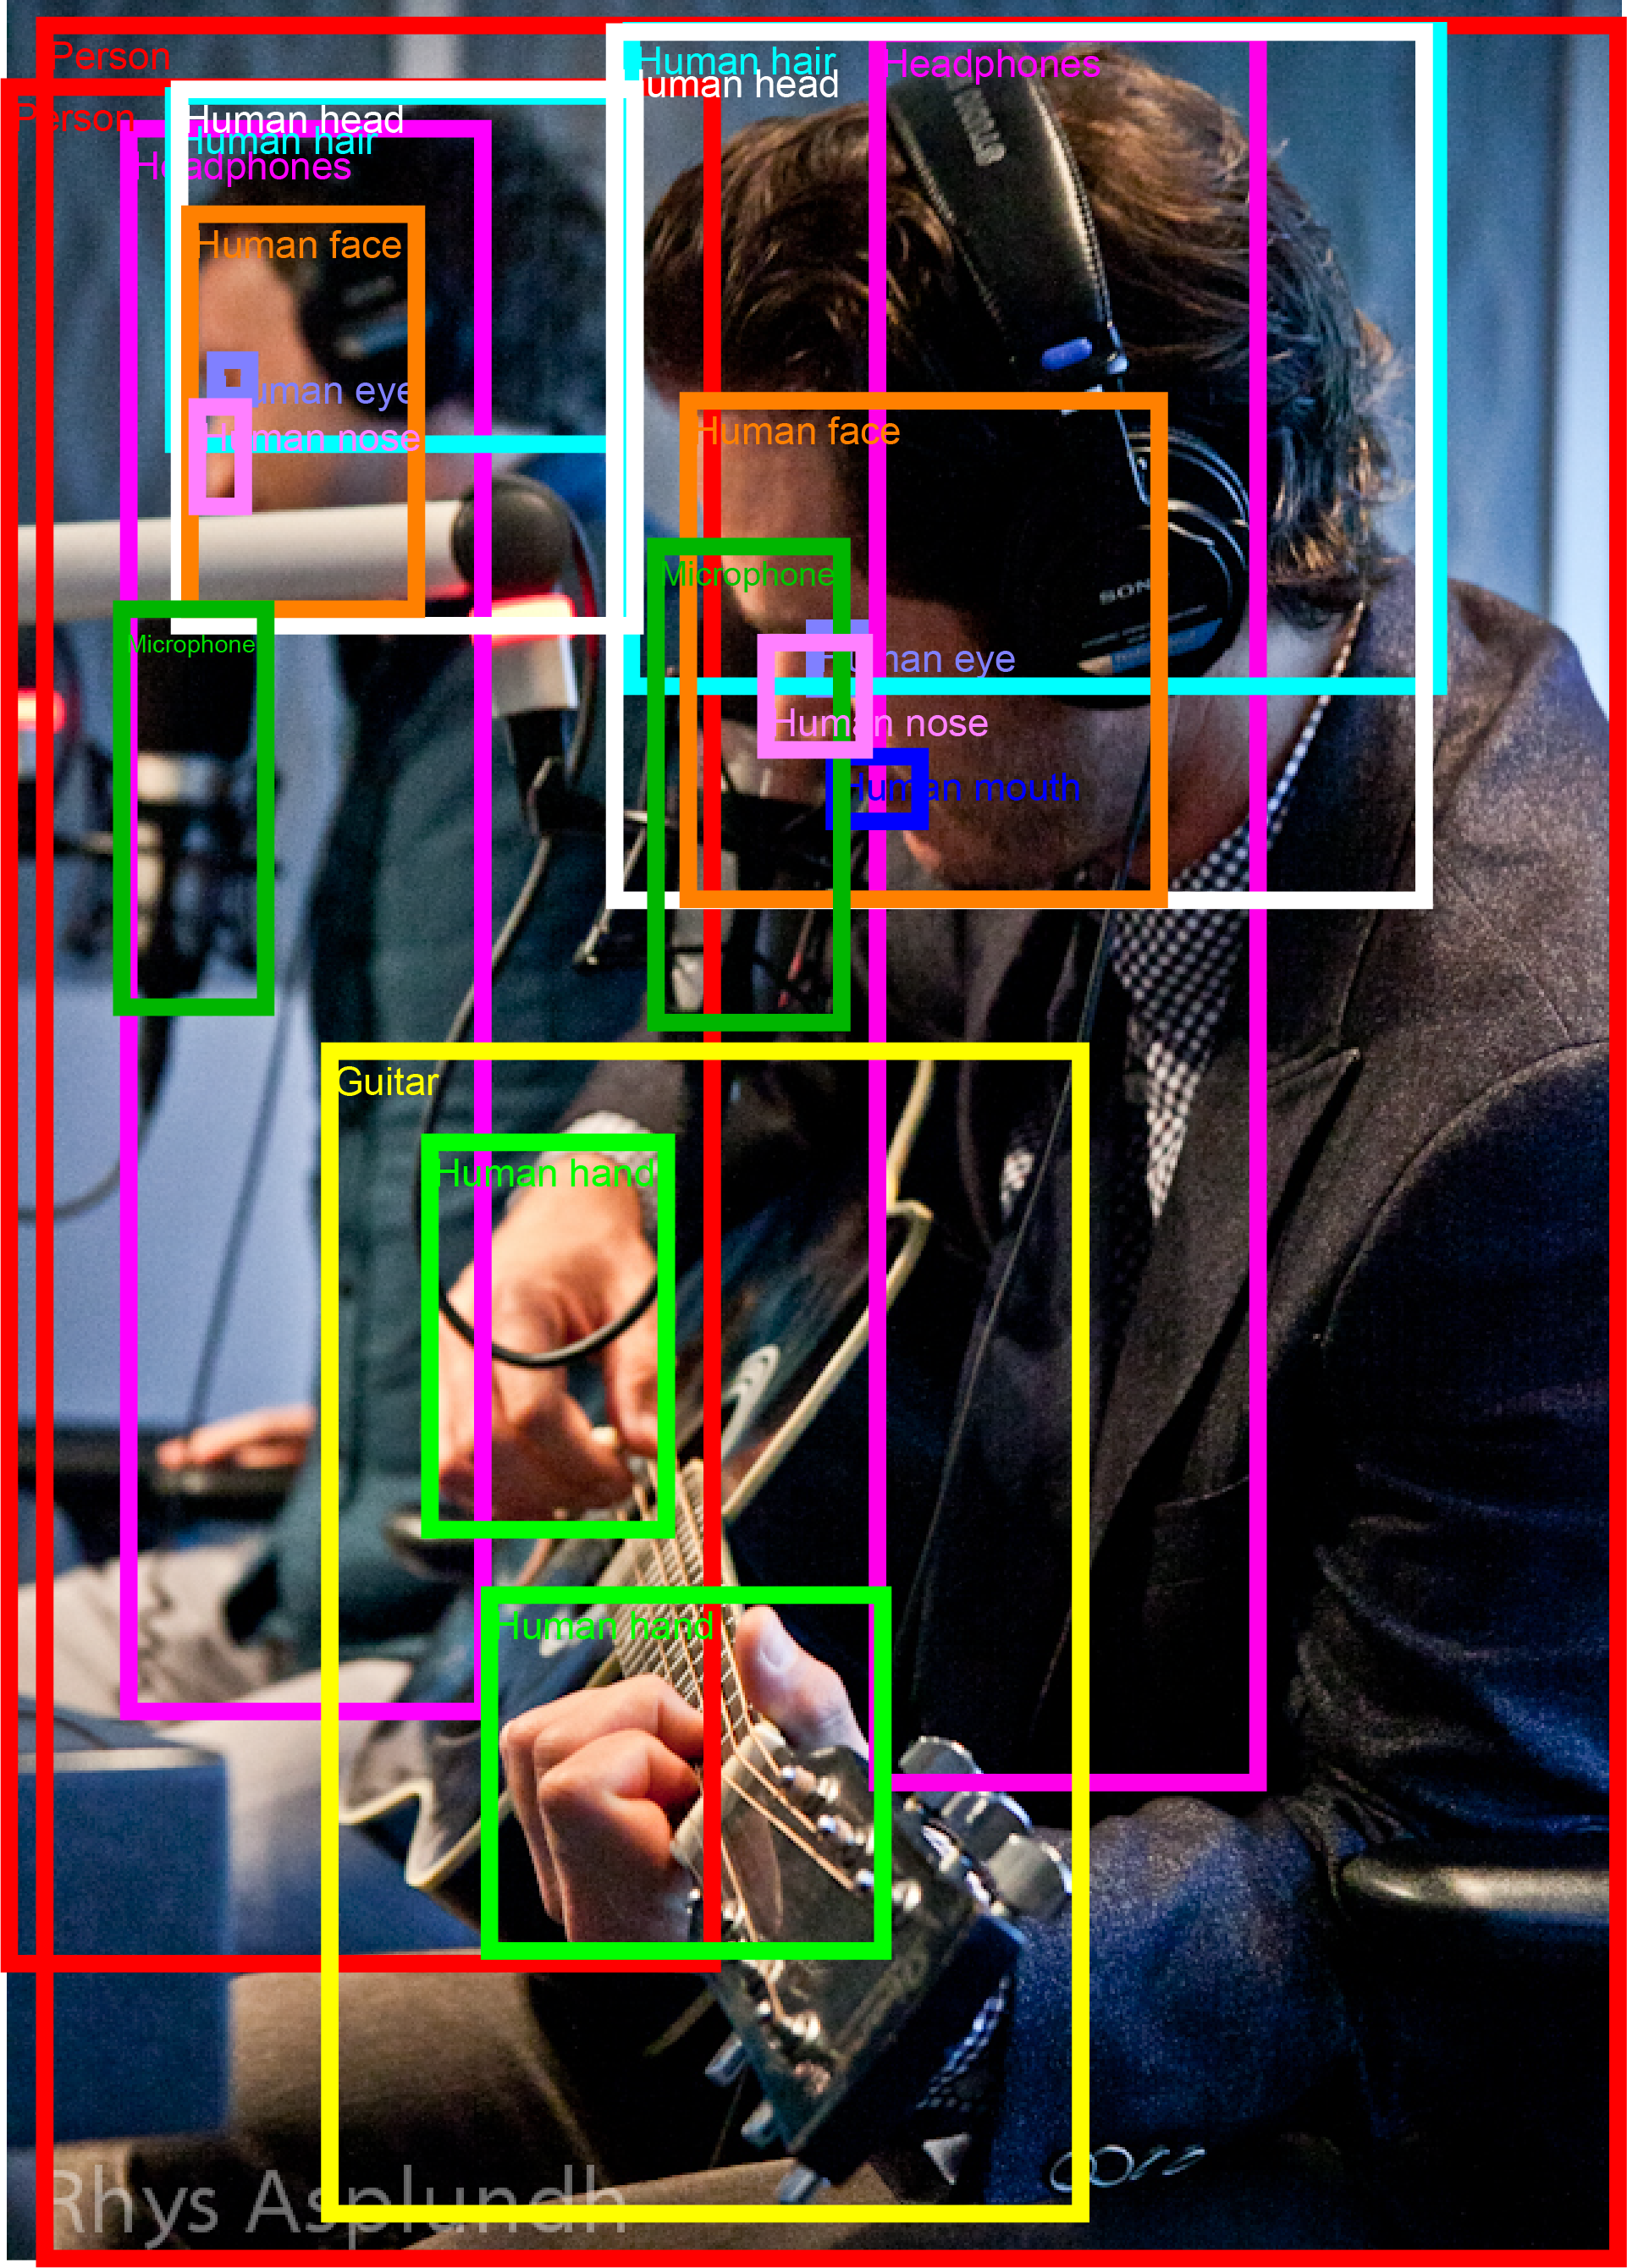
\includegraphics[width=.7\textwidth]{intro-1.png}
	\caption{\scriptsize Mark Paul Gosselaar plays the guitar by Rhys A. \cite{google:1}}
\end{figure}

The Kaggle challenge created by Google called Open Images 2019 - Object Detection \cite{kaggle} motivates this project. This Kaggle was created using the recent data set announced, the Open Images Dataset v5 \cite{google:1}. This project proposes to show some strategies to solve the problem, given a deep dive into some deep neural network architectures. 

\subsection{Problem Statement}
\subsection{Metrics}
\section{Analysis}
\subsection{Data Exploration}
\subsection{Exploratory Visualization}
\subsection{Algorithms and Techniques}
\subsection{Benchmark}
\section{Methodology}
\subsection{Data Preprocessing}
\subsection{Implementation}
\subsection{Refinement}
\section{Results}
\subsection{Model Evaluation and Validation}
\subsection{Justification}
\section{Conclusion}
\subsection{Free-Form Visualization}
\subsection{Reflection}
\subsection{Improvement}

\bibliographystyle{unsrt}
\bibliography{references.bib}{}
\end{document}